% !TeX root = ../libro.tex
% !TeX encoding = utf8
%
%*******************************************************
% Introducción
%*******************************************************

% \manualmark
% \markboth{\textsc{Introducción}}{\textsc{Introducción}} 

\chapter{Introducción}

En el ámbito matemático, cuando se define una estructura ligada a un elemento, la pregunta natural es si siempre es posible encontrar una para un elemento concreto (existencia) y en caso de que exista, si es la única bajo ciertas condiciones (unicidad).\\
\begin{wrapfigure}{r}{3cm}
	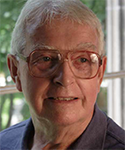
\includegraphics[width=3cm]{munkres_james}
	\caption*{J. R. Munkres.}\label{wrap-fig:munkres_james}
	\vspace{2.2cm}
	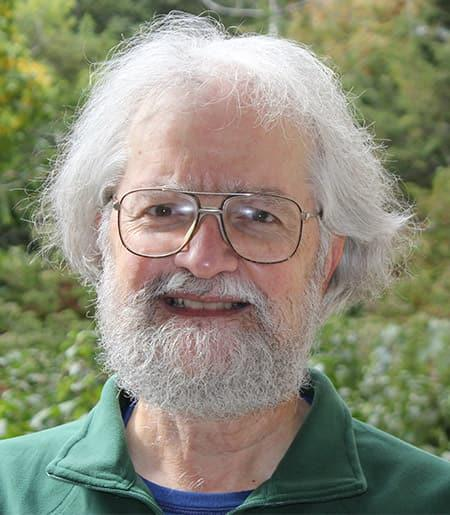
\includegraphics[width=3cm]{allen_hatcher}
	\caption*{Allen Hatcher.}\label{wrap-fig:allen_hatcher}
\end{wrapfigure} 
\\Un problema clásico de la topología diferencial es si es posible definir para toda superficie topológica una única estructura diferenciable salvo difeomorfismos. J. R. Munkres lo demostró en su tesis doctoral (1955) utilizando que toda superficie topológica admite una triangulación diferenciable, junto con ciertas técnicas analíticas sofisticadas.\\
\\Dicha cuestión ha estado ligada a la clasificación de estructuras lineales a trozos, para variedades topológicas $n$-dimensionales. En $1960$, Kirby y Shiermann usaron una técnica novedosa en ese campo, el ``Truco del Toro'' de Kirby, para demostrarlo en dimensiones superiores. Más tarde, esta técnica fue adaptada por A. J. S. Hamilton en $1976$, demostrando de nuevo los resultados sobre existencia y unicidad de estructuras lineales a trozos en variedades tridimensionales aportados por Moise. Parte de esta información se puede encontrar en la introducción que hace J. R. Munkres en su artículo ``Obstructions to Imposing Differentiable Structures'' \cite{Munkres} y la recopilación histórica de Ciprian Manolescu \cite{Historical}.\\
\\Lo que consigue Allen Hatcher en su artículo \cite{arXiv:1312.3518} es trasladar la técnica del toro de Kirby a variedades topológicas $2$-dimensionales, enunciando y demostrando $2$ resultados cuyo corolario trivial es el teorema de existencia y unicidad para el caso de superficies topológicas.\\
\\Cabe destacar que el teorema deja de ser cierto para estructuras de mayor complejidad, como la conforme y la isométrica, he incluso para variedades de dimensión $n \geq 3$.\\
\\Para comprender la importancia del problema de suavizar una ``estructura topológica'', se ha propuesto el estudio de la realización de una buena aproximación a una superficie, gestionando los recursos de manera eficiente para su visualización en tiempo real. Además, permitirá la visualización de homotopías a modo de animaciones fluidas.\\
\\Actualmente estamos observando el auge del hardware para renderizado mediante trazados de rayos, muy útil para la correcta representación de una superficie (bajo un cierto margen de error), pero está lejos de las capacidades de un computador medio si se quiere ejecutar en tiempo real. Es por ello que se ha orientado el estudio al uso de mallas, es decir, aproximar una superficie mediante un conjunto de triángulos, para renderizar mediante rasterizado. El estudio en sí consistirá en detectar en qué zonas será necesaria una mayor cantidad de triángulos para aproximarla mejor.\\
\\Antes de iniciar el estudio del teselado (subdivisión de triángulos) será necesario definir un lenguaje propio para poder indicar explícitamente las cartas de la superficie. Se realizará por medio de un ``procesador'' que dará como salida un código GLSL, que se incluirá en los shaders donde sea necesario. Este programa no funcionará sólo como traductor, sino que tiene el objetivo principal de obtener los árboles de expresión de las funciones definidas y ser capaz de calcular los árboles de las derivadas parciales, para obtener las funciones típicas de una superficie (normal, curvatura, etc).\\
\\Inicialmente se propuso el uso del Geometry shader para implementar un algoritmo de teselado propio, ya que el Geometry shader requiere una versión no muy reciente de OpenGL y aportaría mayor flexibilidad. Sin embargo, por algunas causas que se comentarán en apartado de \textbf{Implementación y pruebas}, decidí utilizar el Tessellation shader, que es más reciente y está diseñado específicamente para el teselado, incrementando considerablemente el rendimiento de la aplicación.\\
\\El problema a tratar es la explicación de la prueba de existencia y unicidad, salvo difeomorfismos, de una estructura diferenciable para toda variedad topológica 2-dimensional sin bordes, de manera que un estudiante del grado de Matemáticas lo entienda con claridad, siempre que suponga ciertos los resultados utilizados de la teoría de Morse. También se diseñará he implementará un programa capaz de visualizar una superficie por cartas, mediante rasterizado, gestionando correctamente los recursos. Además, se ha conseguido incluir la posibilidad de utilizar derivadas parciales de funciones definidas por el ususario y la visualización de funciones de Morse por niveles (isobaras) junto con sus puntos críticos (actualmente sólo para la función de Morse ``altura'').

\section*{Contenido de la memoria}
El trabajo, sin contar las secciones comunes, se ha dividido en $2$ partes, una para la demostración del teorema central (parte matemática) y otra para el estudio de visualización de superficies (parte informática). Cada parte tiene un capítulo dedicado a los conceptos básicos utilizados, para orientar al lector.
\begin{itemize}
	\item Para la parte matemática, el capítulo que trata los conceptos básicos se complementará con otro en el que se indiquen los resultados más importantes utilizados.
	\item En cuanto a la parte informática, se han añadido los capítulos referentes al desarrollo de una aplicación (capítulos 7, 8 y 9), aunque cabe destacar que ha tenido bastante peso el estudio de la teselación, por lo que algunos diagramas no se indicarán si no son relevantes. Es decir, el diseño de la aplicación en sí ha sido el más sencillo posible, para dedicar el mayor tiempo posible a la teselación, eficiencia, robusted y portabilidad de la aplicación.
\end{itemize}
Se han añadido como apéndices una \textbf{Guía de instalación}, donde además se indicarán los requisitos previos, y una \textbf{Guía de uso}.

\section*{Fuentes principales}
Como principales fuentes de información para la realización del proyecto, se han consultado las siguientes referencias:
\begin{itemize}
	\item En la demostración del teorema, los artículos de Allen Hatcher \cite{arXiv:1312.3518} y \cite{MorseTh1}.
	\item Para la implementación del programa, la documentación de OpenGL en la Wiki de Khronos \cite{KhronosWiki} y la de Dear ImGui para la interfaz \cite{ImGui}.
\end{itemize}

\endinput
